\section{Prototypes}\label{sec:prototypes}

As a first (\texttt{v1}) prototype of this capability, a standalone columnar implementation of the ATLAS Egamma CP tool with zero-copy \texttt{nanobind} Python bindings was created to compute on-the-fly systematics variations for the dilepton system mass in $e^{+}e^{-}$ final states, $m_{ee}$.
Uproot was used to load PHYSLITE files of ATLAS $Z\to \ell\ell$ simulation into Awkward arrays, and the $e^{+}e^{-}$ event selections were applied with Coffea.
The columnar Egamma tool was initialized through the Pythonic interface, \texttt{atlascp.EgammaTools}, and then passed Awkward arrays of electrons to compute on-the-fly systematic variations of the electron reconstruction efficiency scale factors and energy correction resolution and scale.
The computations were additionally scaled out with \texttt{dask-awkward}~\cite{dask_awkward_2024} on the University of Chciago ATLAS Analysis Facility to minimize the compute wall time, with the gathered results visualized in~\Cref{fig:Zee_mc_systematics}.

This \texttt{v1} prototype established foundations of what was possible with new tooling and that Pythonic interfaces to CP tools could be written without large amounts of work or deep knowledge of underlying CP tool design.
This was promising, but additional work was needed to achieve necessary performance required for use.
Though as there was no ``zero action'' option --- some amount of research was required to determine the viability of the proposed design --- this prototype was valuable.

Following this work, a \texttt{v2} ``Columnar Athena'' prototype~\cite{columnar_athena} has been started to expand the scope of the work.
This moves the development of the columnar CP tools and interfaces from standalone examples into the ATLAS Athena framework~\cite{ATLAS_Athena} and migrates the ATLAS CP tools to a columnar backend with breaking the existing workflows using the EDM models.
It additionally adds infrastructure support for development of columnar analysis tools by adding \texttt{nanobind} to the ATLAS Externals tooling distributed as part of the ATLAS Athena Analysis Releases.
While currently under active development, the \texttt{v2} prototype will allow for full scale integration and performance tests of the columnar CP tools and interfaces.

\begin{figure}
    \centering
    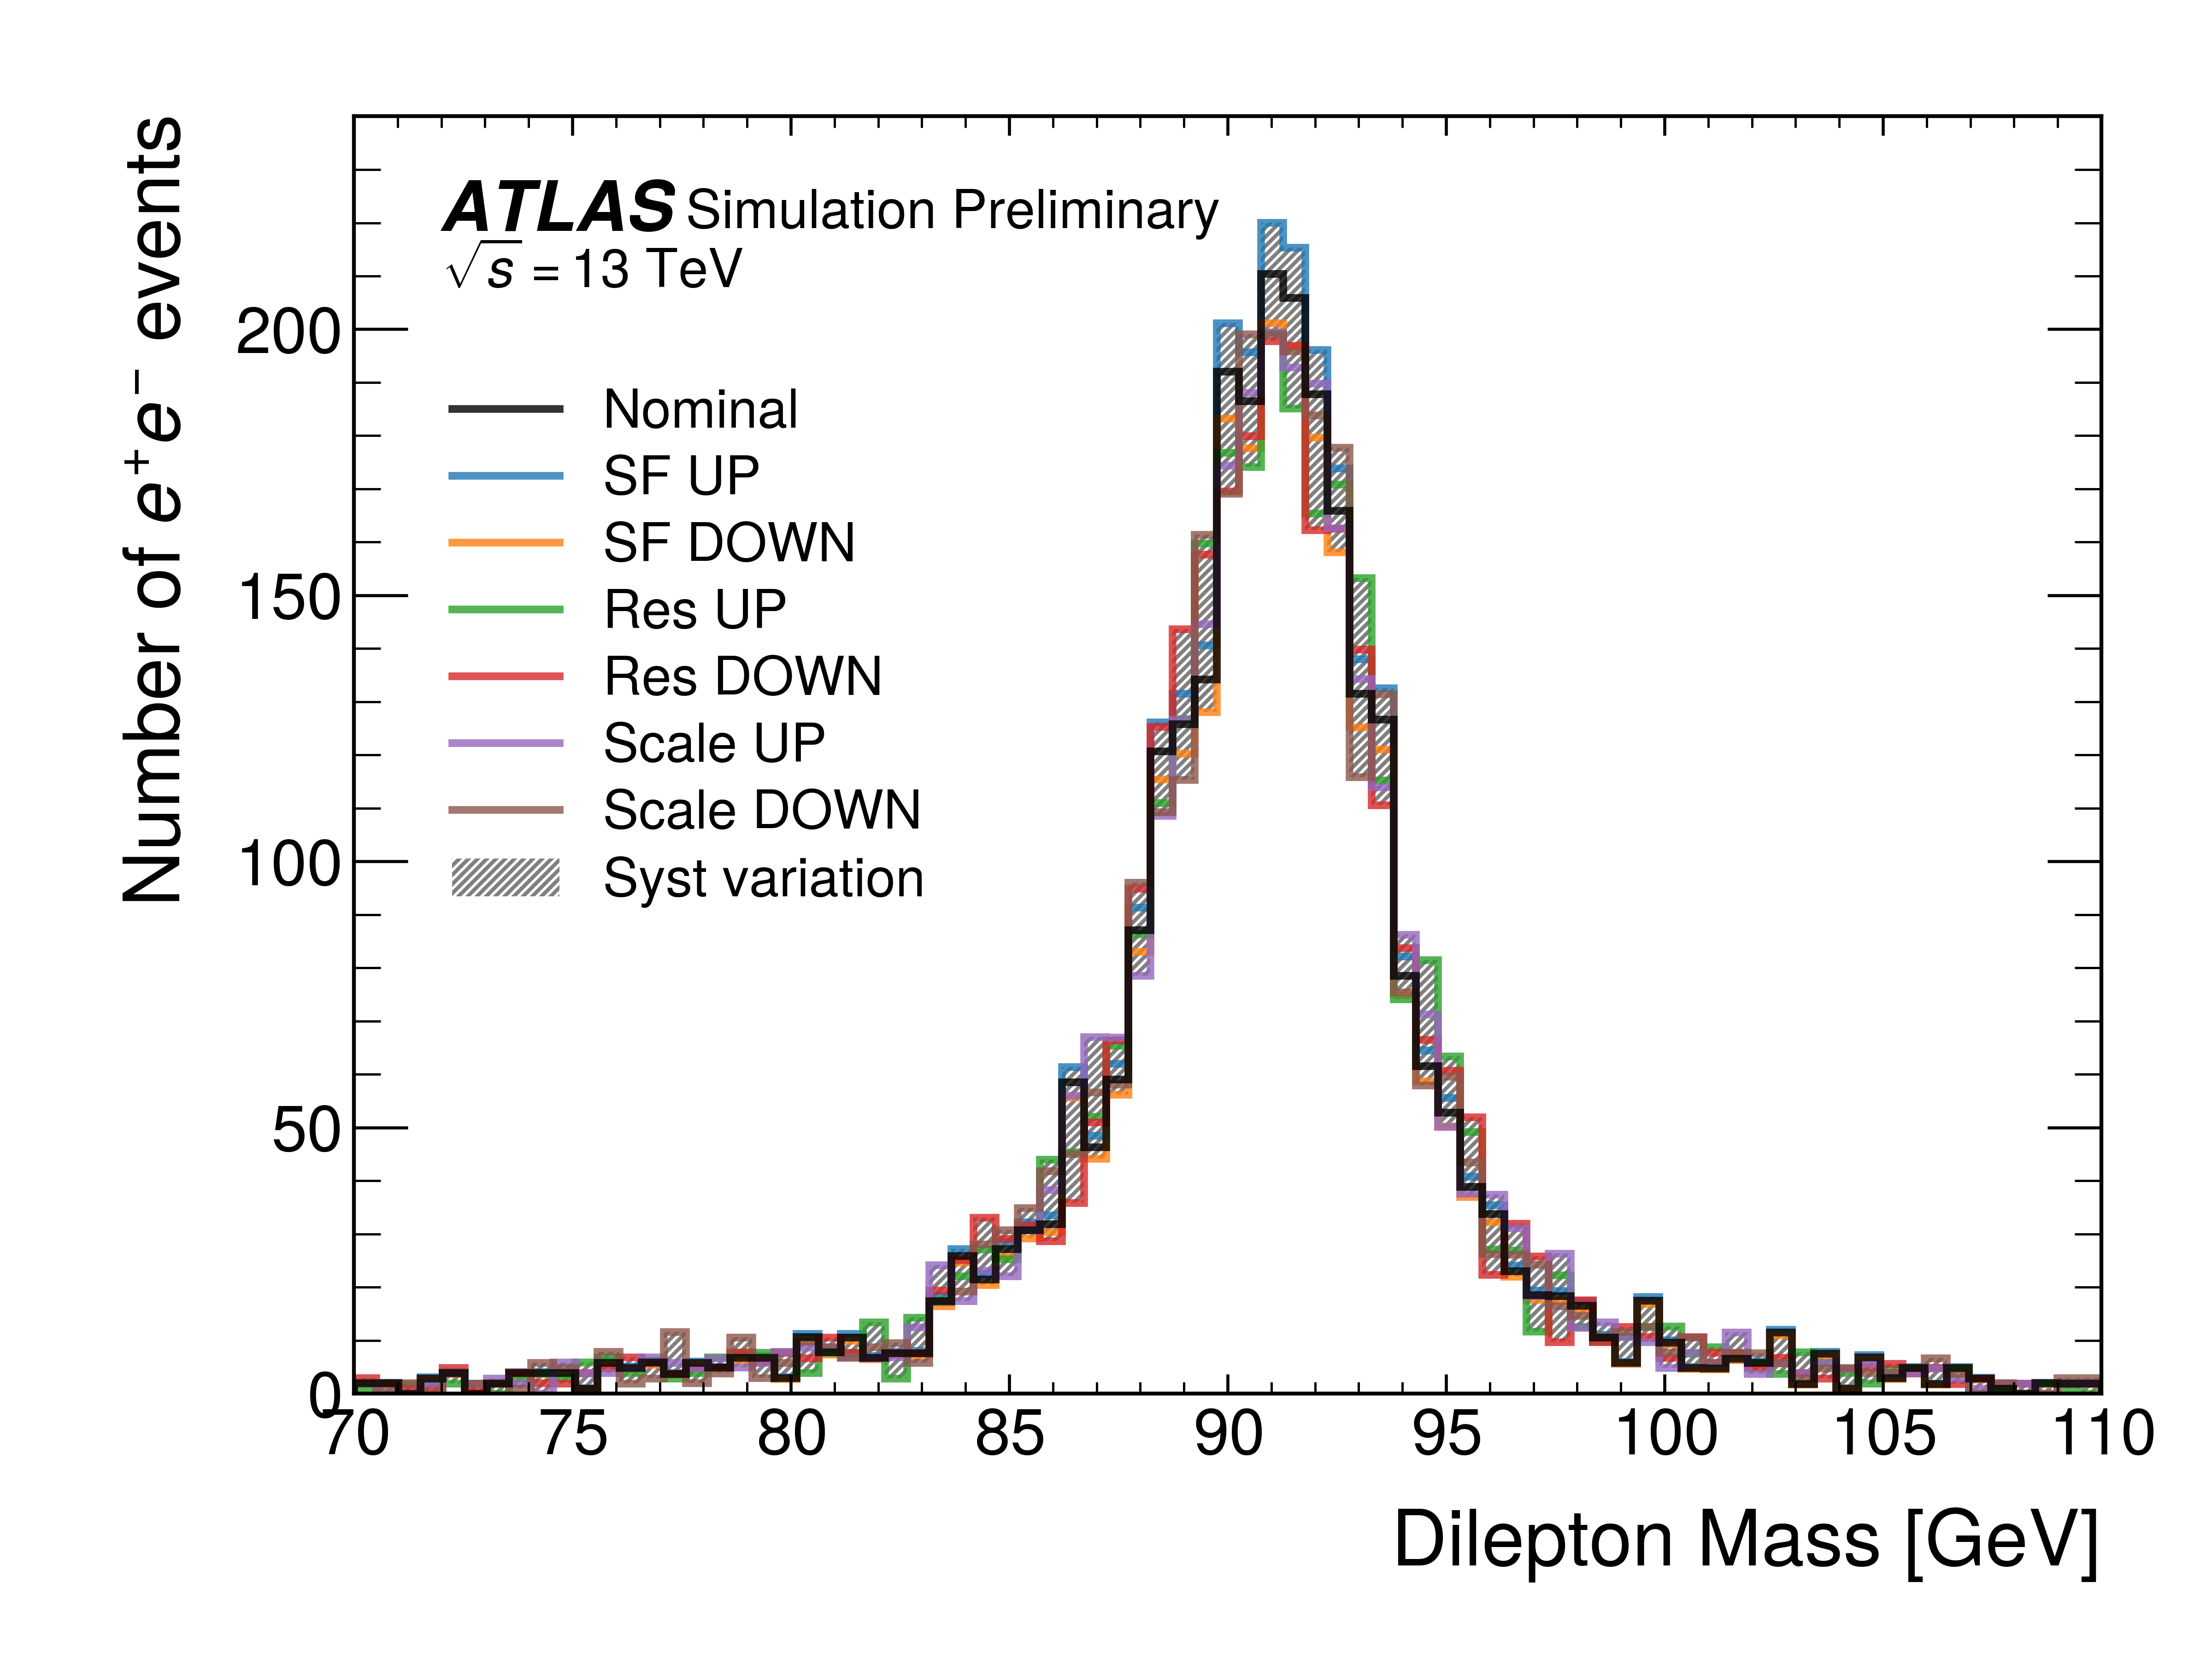
\includegraphics[width=0.7\textwidth]{Zee_mc_systematics.png}
    \caption{Selected $m_{ee}$ under on-the-fly computed systematic variations of electron reconstruction efficiency and corrections~\cite{Vigl:ACAT_2024}.}
    \label{fig:Zee_mc_systematics}
\end{figure}
